\section{研究现状}
\label{sec1:related}
在上一节的内容中,我们回顾了过去十年间人工智能(AI)和自然语言处理(NLP)领
域所取得的显著进展,并探讨了常识性知识领域的进步如何为常识性推理研究提供重要支撑。
此外,我们还分析了在这常识性推理领域所面临的挑战,概述了我们在应对这些挑战时主要的研究内容和贡献。
为本章内容的深入探讨奠定了基础。本章旨在全面介绍常识性推理的研究现状,
涵盖从主要任务和评估基准到近年来流行的方法和模型,以及这些模型在可
解释性和鲁棒性评估方面的研究进展。

本章首先聚焦于常识性推理领域的核心任务及其相关评估基准(benchmarks),以
此为出发点,探讨了任务的具体内容、目标和挑战。随后,我们将深入讨论推理模型
的方法论,包括符号方法、早期统计方法以及神经网络方法,并详细分析这些方法的
优势和局限性。这些数据集和推理方法将在后续章节中将被频繁引用。

接下来,本章将重点探讨推理模型鲁棒性的研究。这部分内容包括鲁棒性的定义、测
试方法,以及用于增强模型鲁棒性的各种策略。我们将深入分析模型所面对的多样化和对
抗性数据类型,并探索提升这些模型鲁棒性的有效途径。

最后,本章将探讨推理模型的可解释性研究,包括模型鲁棒性不足现象分析、模型鲁棒性不足的
原因的假设和验证方法。
这一部分的内容对于理解模型在复杂环境下的行为模式及其背后的原因至关重要。

综上所述,本章将为读者提供一个全面而深入的视角,以理解常识性推理领域的当
前研究现状,包括其核心任务、评估基准、方法论以及鲁棒性和可解释性的研究进展。



%在上一节中,我们细致回顾了过去十年间人工智能(AI)和自然语言处理(NLP)领域所取得的重大进步。我们不仅探讨了这些进步对于常识性推理研究的重要性,
%还分析了在这一研究领域中所面临的挑战。本章将深入介绍常识性推理的研究现状。
%我们首先将探讨此领域所涵盖的主要任务及其相关的评估基准(benchmarks),随后,
%会详细讲述近年来流行的方法和模型,以及这些模型在鲁棒性方面的评估方法(包括解释性评估)和提升策略。

\subsection{任务}
\label{sec1:task}


在常识性推理领域,存在多个关键任务\cite{storks2019recent},每个任务都在理解和推动人工智能发展中发挥着至关重要的作用。以下为这些任务的详细介绍:
\begin{enumerate}
  \item \textbf{Reference Resolution(指代消解)}:
  指代消解任务涉及识别文本中特定表达式(如代词或短语)所指代的对象。这一任务对于自然语言处理至关重要,它不仅要求理解语言的上下文,还要求捕捉到语言的隐含意义。复杂句子中的多个名词和代词之间的准确指代关系识别,
  不仅需要深入理解句中实体间的关系和上下文环境,有时更需借助外部常识性知识\cite{morgenstern2016planning,davis2017first}。
  指代消解是理解复杂文本和对话的基础,对于提升机器的语言理解能力至关重要。

  \item \textbf{Question Answering(问题回答)}:
  这个任务要求对特定文本片段进行深入理解,以回答有关该文本的问题。这不仅考验了机器在处理语法和词汇基础上的能力,
  也考验了其在理解文本、提取关键信息、逻辑推理乃至应用外部知识等方面的能力。机器必须能够理解文本的深层含义,
  并在必要时利用广泛的背景知识来进行回答。

  \item \textbf{Textual Entailment(文本蕴涵)}:
  文本蕴涵是由Dagan等人(2005)\cite{dagan2005pascal}定义的,指的是文本与假设之间的方向性关系,其中如果一个典型人根据文本会推断假设为真,
  则可以说文本蕴含假设。一些基准测试通过要求识别矛盾来扩展这项任务,例如第四和第五届RTE挑战\cite{giampiccolo2008fourth,bentivogli2009fifth}。
  与问题回答相似,文本蕴涵任务需要利用多种简单的语言处理技能,例如命名实体识别和共指解析。
  不同于问题回答,文本蕴涵还需要理解一个典型人可能做出的推断,因此常识性知识对于这个任务至关重要。

  \item \textbf{Plausible Inference(合理推理)}:
  Davis和Marcus(2015)\cite{davis2015commonsense}定义的合理推理任务要求系统在有限上下文中做出合逻辑的、中间性的或不确定性的结论。
  这涉及到在故事中断的关键时刻,选择或生成最合理的后续事件。系统不仅需理解给定信息,
  还需运用常识性知识和逻辑推理预测最可能的结果。

  \item \textbf{Intuitive Psychology(直觉心理学)}:
  %\Shan{注意这里ROC举的例子}
  直觉心理学是合理推理任务中的一个重要领域,涉及通过行为推断情感和意图,这是人类的一项基本能力。
  有些基准测试在某些示例中涉及这个主题。%例如ROC\cite{mostafazadeh2016corpus}在表\ref{tab:table1}中的求婚例子,
  直觉心理学任务集中于理解和推断人类行为背后的动机、情感和意图。系统需要理解文本中的事实信息,并对人物的心理状态和社会互动进行深刻洞察。

  \item \textbf{Multiple Tasks(多任务)}:
  一些基准测试由几个单独的语言处理或推理子任务组成,以便在统一的格式下学习和测试不同的阅读理解技能,
  比如bAbI\cite{weston2016towards}和GLUE\cite{wang2018glue}。这些基准可以用作诊断工具,
  以确定模型在不同领域的表现。子任务通常是从各种已存在的基准测试中重新框定的\cite{white2017inference}。
  这些基准对于全面评估和提高人工智能系统的语言处理能力至关重要。
\end{enumerate}

\subsection{基准数据集}
\label{sec1:benchmarks}
%\Shan{注意之后所有arct\_adv改成STS}
%在探索常识性推理领域时,本文重点关注了\secref{sec1:task}所提及的若干关键任务。
%这些任务对于理解和推进人工智能的发展起着至关重要的作用。特别地,本节深入探讨了与这
%些任务紧密相关的主要数据集。这些数据集不仅为研究者提供了丰富的实验资源和标准化评估基准,
%而且直接映射出当前自然语言处理技术的成就与挑战。下面的表格(\tabref{tab1:datasets})列出
%了与各种任务类型相关的关键数据集。

在探索常识性推理领域时,我们特别关注了\secref{sec1:task}中提及的若干关键任务,
每个任务都在理解和推动人工智能发展方面扮演了至关重要的角色。本小节重点介绍了
与这些任务紧密相关的主要数据集。这些数据集不仅为研究提供了丰富的实验材料和
标准化的评估基准,还直接反映了当前自然语言处理技术的发展水平及其面临的挑战。
下面的表格(\tabref{tab1:datasets})详细展示了各种任务类型相关的关键数
据集,包括SNLI\cite{bowman2015large}、MNLI\cite{williams2018broad}、
QNLI\cite{wang2018glue}、COPA\cite{roemmele2011choice}、
ROC\cite{mostafazadeh2016corpus}、SWAG\cite{zellers2018swag}、
RACE\cite{lai2017race}、RECLOR\cite{yu2020reclor}、
FEVER\cite{thorne2018fever}、
STS\cite{schuster2019towards}、
ARCT\cite{habernal2018argument}、
CQA(CommonsenseQA)\cite{talmor2019commonsenseqa}和
Ubuntu\cite{lowe2015ubuntu}。


接下来,我们将对\tabref{tab1:datasets}中提到的每个数据集的格式以及其主要特点进行详细介绍,
以更深入地理解它们在评估不同推理任务中的作用和重要性。

\begin{table}[th!]
  \centering
  \scriptsize
  \begin{tabular}{
  >{\centering\arraybackslash}p{0.15\textwidth}|
  >{\centering\arraybackslash}p{0.20\textwidth}|
  >{\centering\arraybackslash}p{0.10\textwidth}|
  p{0.28\textwidth}}
      \toprule
      \textbf{数据集} & \textbf{任务类型} & \textbf{任务格式} & \textbf{特点} \\ 
      \midrule
      SNLI & 文本蕴涵 & 分类 & 成对句子判断蕴涵关系 \\ 
      \midrule
      MNLI & 文本蕴涵 & 分类 & 多体裁文本蕴涵 \\ 
      \midrule
      QNLI & 文本蕴含,问题回答 & 分类 & 问题与回答的判断 \\ 
      \midrule
      ROC & 合情推理 & 多项选择 & 选择故事合理结尾 \\ 
      \midrule
      COPA & 合理推理 & 多项选择 & 因果或效果的选择 \\ 
      \midrule
      SWAG & 合情推理 & 多项选择 & 预测情境后续 \\ 
      \midrule
      RACE & 合情推理 & 多项选择 & 中高中水平阅读理解 \\ 
      \midrule
      RECLOR & 合情推理 & 多项选择 & 逻辑推理阅读理解 \\ 
      \midrule
      FEVER & 合理推理 & 分类 &用于评估模型在事实验证方面的能力 \\ 
      \midrule
      STS & 合情推理 & 分类 &  测试声明和相应证据的准确性\\ 
      \midrule
      ARCT & 问题问答 & 分类 & 论证有效性评估 \\ 
      \midrule
      CQA & 问题问答 & 多项选择 & 评估常识性知识理解 \\ 
      \midrule
      Ubuntu & 问题问答 & 多项选择 & 对对话模型的评估 \\
      \bottomrule
  \end{tabular}
  \caption{常识性推理数据集概览。}
  \label{tab1:datasets}
\end{table}




%接下来,我们将对\tabref{tab1:datasets}中提到的每个数据集进行更深入的介绍,以便更好地理解它们在各自任务中的应用和重要性
1. SNLI(Stanford Natural Language Inference):
如\tabref{tab1:datasets}所示,Stanford Natural Language Inference(SNLI),
由Bowman等人于2015年提出(参见文献\cite{bowman2015large}),是一项基准测试。它包含近60
万个句子对,旨在执行类似于第四和第五届RTE挑战(参见文献\cite{giampiccolo2008fourth,bentivogli2009fifth})
的三种推理任务。除了标准的蕴涵、矛盾和中立标签,SNLI数据集还特别包含了五种群体判断标签,
这些标签反映了对每个判断的信心程度和一致性水平。

2. MNLI(Multi-Genre Natural Language Inference): 
由Williams等人提出\cite{williams2018broad},包含433,000个示例,是目前最大的自然语言推理语料库之一。
它涵盖了十种不同体裁的书面和口语英语,旨在涵盖现代标准美国英语使用的全部多样性。
所有体裁都出现在测试和开发集中,但只有五种体裁包含在训练集中。
这种设计允许研究者评估模型在已知来源(匹配)和未知来源(不匹配)的测试示例上的表现。
MNLI数据集的目的是推动自然语言理解(NLU)领域的研究,特别是在领域适应和跨领域转移学习方面。

3. QNLI(Question Natural Language Inference)数据集\cite{wang2018glue}: 
是基于SQuAD(Stanford Question Answering Dataset)\cite{rajpurkar2016squad}构造的,
SQuAD由Rajpurkar等人(2016)提出,
专注于自然语言理解和问题回答任务。
SQuAD包含超过10万个问题,旨在从Wikipedia文章段落中找到问题的答案。
QNLI从SQuAD中提取段落和问题,转换成自然语言推理的形式,
即给定一个声明(问题)和一个文本片段(段落),要求模型确定文本是否包含该声明的答案。
这种转换允许QNLI评估模型在理解复杂文本及其隐含含义的能力,尤其是在深入分析和推理的背景下。

4. COPA(Choice of Plausible Alternatives)\cite{roemmele2011choice}: 由Roemmele等人在2011年提出,是一个专注于评估事件之间因果推理的任务。
这个任务需要常识知识来判断通常在世界上发生的事件。COPA提供一个前提和两个选择,
要求从中选择一个作为最合理的原因或效果,测试模型的向前或向后因果推理能力。
数据集包含1,000个这样的实例,是评估模型在理解和推理因果关系方面的能力的重要工具。

5. ROC\cite{mostafazadeh2016corpus}: 由Mostafazadeh等人在2016年提出,是一个专注于日常生活故事的语料库,包
含大约50,000个五句话故事。这些故事涵盖了丰富的因果和时间关系,
非常适合于学习和评估常识性知识。其中大约3,700个故事被指定为测试用例,
每个测试案例包含一个合理和一个不合理的备选故事结尾,供模型在故事闭幕测试中进行选择。
这个测试是Chambers和Jurafsky(2008)提出的
叙事任务\cite{chambers2008unsupervised}的一个更具挑战性的替代方案,
旨在评估模型理解故事情节和进行逻辑推理的能力。

6. SWAG(Situations With Adversarial Generations)\cite{zellers2018swag}: 由Zellers等人(2018)提出,
是一个包含大约113,000个文本开头的基准数据集,每个文本开头有四个可能的结尾。
这个基准测试旨在评估模型在情境推理方面的能力。

7. RACE数据集\cite{lai2017race}: 由Lai等人在2017年开发,
是一个专为评估模型在阅读理解任务上的能力而设计的挑战性数据集。
它包含了来自中国中学和高中英语考试的28,000篇文章,共计约98,000个多项选择题。
这些问题不仅覆盖了广泛的主题,而且往往设计得非常巧妙和具有挑战性,
经常要求对文章中的多个句子或段落进行深入推理。与一般的阅读理解数据集不同,
RACE中的问题和候选答案通常无法通过简单的文本匹配直接找到答案,
而是需要模型进行高级的推理和理解,这使得RACE成为评估和提升自然语言理解系统的一个重要工具。

8. RECLOR数据集\cite{yu2020reclor}: 由Yu等人于2020年提出,
旨在评估逻辑推理能力在阅读理解中的应用。
该数据集从标准化的研究生入学考试(如GMAT和LSAT)中提取了6,138个逻辑推理问题,
每个问题都包括一个上下文段落、一个问题和四个选择答案,其中只有一个是正确的。
RECLOR的设计特点是它要求模型不仅理解给定文本,还需要进行深入的逻辑推理,
以便在多个选择中找到正确答案。这种设计使RECLOR成为一个具有挑战性的数据集,
用于测试和提高自然语言处理模型在复杂逻辑推理方面的能力。

9. FEVER\cite{thorne2018fever}: 由Thorne等人于2018年提出,是一个大规模的事实提取和验证数据集。
该数据集包含185,445个声明,这些声明是通过修改从Wikipedia提取的句子生成的,
并在没有句子原文的情况下进行了验证。声明被分为三类:支持(Supported)、
反驳(Refuted)或信息不足(NotEnoughInfo),由标注者进行分类,
其一致性达到0.6841 Fleiss kappa。对于前两类,标注者还记录了形成其判断所需的证据句子。
FEVER数据集的设计旨在提供一个挑战性的测试平台,帮助推动针对文本来源的声明验证领域的进步。
该数据集通过对声明和正确证据的标注实现了31.87%的最高准确率,而如果忽略证据,
准确率达到50.91\%

10. STS(Symmetric Test Set)\cite{schuster2019towards}: 旨在解决在流行的FEVER\cite{thorne2018fever}数据集中出现的偏见问题。
由Schuster等人提出,这个新的``Symmetric Test Set''
包含956个声明-证据对。每个原始声明-证据对都被人工生成了一个具有相同关系(
支持或反驳)但表达不同、相反事实的合成对。这个测试集的构造完全消除了模型仅依赖于声明中线索的能力。

11. ARCT(Argument Reasoning Comprehension Task)\cite{habernal2018argument}: 由Habernal等人于2018年提出,
专注于评估模型在理解和分析论证性文本方面的能力。
该数据集提供了在线新闻文章评论中的论证结构,包括约2,500个例子。
每个例子包含一个观点、一个支持或反对该观点的论据,以及两个备选的保证(warrant),
其中只有一个能正确地支持论证。任务是识别出正确的保证。ARCT的挑战在于,
许多论证的保证并非直接表达,而是隐含在论证中,需要模型通过外部知识进行推断。
这种设计使ARCT成为一个有价值的工具,用于推动自然语言处理模型在理解、
分析和推理论证性文本方面的进步。

12. CQA是CommonsenseQA\cite{talmor2019commonsenseqa}数据集的缩写,由Talmor等人于2019年提出,是一个针对常识性知识的问答(QA)基准测试。它
包含9,500个三项选择问题,旨在测试模型在解决涉及常识性推理的问题上的能力。
每个问题都要求从ConceptNet这一常识性知识图中的三个相连概念中消除一个目标概念的歧义。
CommonsenseQA的设计确保了问题不仅直接针对常识性关系,而且所需的常识性知识领域对日常使用
来说相当全面,从而在自然语言处理领域中提供了一个具有挑战性的评估基准。

13. Ubuntu对话语料库\cite{lowe2015ubuntu}由Lowe等人创建,是一个大规模的多轮对话数据集,
用于研究非结构化对话系统。该数据集包含近100万个对话,超过700万次发言,
以及1亿个词汇。这些对话来源于2004年至2015年间的Ubuntu聊天日志,
主要用于技术支持和问题解答。Ubuntu对话语料库结合了对话状态跟踪挑战数据集中的多轮
对话特性以及类似Twitter等微博服务的非结构化交互特性,为基于神经网络的对话系统研究提供了
丰富的实验资源。

\subsection{推理模型和方法}
\label{sec1:approachs}
为了有效地解决\secref{sec1:task}和\secref{sec1:benchmarks}中所述的基
准任务和数据集挑战,研究者们已经开发出了多样化的方法。这些方法的
发展覆盖了从初期的符号逻辑与统计方法,到近年来深度学习和神经网络技术的广泛应用。
本节旨在简要概述早期的符号逻辑和统计方法,同时将更加深入地讨论在当前和历史基准任务中
广泛采用的代表性神经网络方法,展现它们在现代智能系统推理能力形成中的核心作用。

\subsubsection{符号方法}
符号方法在自然语言推理的应用源起于古典逻辑和演绎推理理论,
如亚里士多德的逻辑理论(亚里士多德,1989)\cite{smith1989prior},并逐渐
发展至现代数学逻辑,例如摩根(1847)\cite{de1847formal}和
布尔(1854)\cite{boole1854investigation}提出的形式逻辑框架。
这些方法依靠逻辑形式和推理过程,对人类智力和推理能力的理解产生了深刻影响。
在人工智能和语言学领域,例如麦卡锡(1968)\cite{mccarthy1959programs}和
Lakoff(1970)\cite{lakoff1970linguistics}的研究,符号方法为机器
的常识推理和语言的语义表示奠定了基础。此外,符号方法也在处理语言问题上显示出
独特价值,如Peirce(1883)\cite{peirce1883theory}提出的逻辑归纳方法
和贝叶斯网络\cite{dechter2013reasoning}。

符号方法在初期RTE挑战中的应用取得了显著成就。例如,Raina、Ng和Manning(2005)\cite{raina2005robust}的研
究通过将句子转化为逻辑形式,并使用逻辑规则与手工编写的映射进行推理,实现了高准确率。然
而,这种方法在大规模数据集的应用上存在局限性,因为手动编写的逻辑规则和映射难以涵
盖语言和语义现象的广泛多样性\cite{kamath2018survey}。

\subsubsection{早期统计方法}
自20世纪90年代中期至2010年代初,统计方法在自然语言处理领域占据了主导地位。
这些方法依赖于精心设计的工程特征和传统统计模型,如决策树\cite{ng2000machine}和朴素
贝叶斯分类器\cite{glickman2006applied}。它们被广泛应用于从词汇特征到更复杂的语
言特征分析,在RTE挑战中所展现的是这些统计方法在理解和解析语言现象方面的潜力和
效果\cite{dagan2005pascal,haim2006second}。

早期统计方法的重大贡献在于它们为理解语言现象提供了基础框架。然而,它
们在处理大规模和高复杂度数据集时表现欠佳。这些方法的性能通常仅略高于随机猜测,
其效率受限于特征工程的复杂度和数据的多样性\cite{haim2006second,lai2014illinois}。尽
管早期统计方法为深度学习方法的发展奠定了基础,但它们在理解语言的深层结构和复杂性方面逐渐显得不足。

\subsubsection{神经网络方法}
神经网络方法在自然语言处理领域,特别是在自然语言推理任务中,
代表了从早期的基于统计方法到复杂神经网络架构的显著进步。这一转变得益于大数据的可用性,
它促使研究人员能够开发并训练更大、更深的神经网络模型,这些模型在多个自然语言推理基准测试中
取得了卓越的成绩。\figref{fig1:neuralmodel}展示了自然语言推理任务中一些典型神经网络
模型的关键组成部分,主要包括预训练的语言表征、推理模型的核心架构,以及针对特定任务设计的输出层。

\begin{figure}[th]
\centering\includegraphics[width=4in]{figures/xulun/neuralmodel.eps}
\caption{自然语言推理任务中神经网络模型的关键组成部分。}
\label{fig1:neuralmodel}
\end{figure}

神经网络方法的基石是词或语言的分布式表征,即词向量或(embedding),这些通常通过在大规模文
本语料库上训练神经网络得到。早期的词嵌入模型,如word2vec\cite{mikolov2013distributed}和
GloVe\cite{pennington2014glove},提供的是上下文无关的静态表示。这意味
着无论目标词出现在何种语境中,其嵌入向量都保持固定不变,这在处理词义多样性和
上下文相关性方面存在局限性。

为了克服这些限制,研究者们发展了基于上下文的词表示模
型,如GPT\cite{radford2018improving}和BERT\cite{devlin2018bert}。这些
模型为同一词汇在不同上下文中提供不同的嵌入向量,使得对语言复杂性的捕捉更为精确。
这些预训练模型可以直接用作下游任务的特征,也可针对特定应用场景进行微调。
例如,GPT和BERT模型采用了一种设计,其中只有很少的部分是特定于特定任务的。
这意味着,当这些模型被用于不同的下游任务(如文本分类、问答系统等)时,我们只需
要对模型的最后几层进行少量的调整,比如改变输出层的结构或者修改损失函数,就
能够使模型适应新的任务。这种设计提供了高度的灵活性,允许同一个预训练模型在
多种不同的任务中有效工作,而无需对模型本身进行大规模的重构。

%例如,GPT
%和BERT的最少任务特定参数设计使得在适配不同下游任务时可以通过简单修改最终层和损失函数来灵活调整。

在词嵌入层之上,为了满足不同下游应用的具体需求,研究者们开发了多种网络架构。
其中包括循环神经网络(RNN),如长短期记忆网络(LSTM\cite{hochreiter1997long})和
门控循环单元(GRU\cite{cho2014learning}),以及
Transformer架构\cite{vaswani2017attention}。这些网络架构
的选择依赖于特定任务的性质和要求。

针对不同的任务,这些网络架构的输出层也会有所不同。例如,在分
类任务中,常用的输出层包括线性层或多层感知器(MLP),并结合softmax函数来
生成概率分布,从而实现类别的预测。而在语言生成任务中,通常采用语言解码器(Decoder)来
生成连贯的文本序列。

神经网络方法的发展不仅增强了系统处理语言多样性和复杂性的能力,还推动了深层次语言
理解和推理能力的提升。接下来,我们将详细探讨几种在神经模型领域的经典方法,


\begin{itemize}
  \item 词向量或嵌入的方法:如 \textbf{FastText}\cite{joulin2017bag},
  \item 在词嵌入层之上的特定网络架构:如 \textbf{ESIM}\cite{chen2017enhanced},
  \item 预训练的上下文表示模型:如 \textbf{GPT}、 \textbf{BERT}、
   \textbf{XLNet}\cite{yang2019xlnet} 和 \textbf{RoBERTa}\cite{liu2019roberta}。
\end{itemize}

\subsubsection*{1. 词向量或嵌入的方法:FastText}

FastText结合了简单的线性模型和高效的词嵌入技术,例如层次化Softmax和n-gram特征,以有效地处理文本分类任务。

1)模型架构
%\Shan{这里有个fasttext的图}

\begin{figure}[th]
  \centering\includegraphics[width=4in]{figures/xulun/fasttext.eps}
  \caption{FastText模型架构。}
  \label{fig1:fasttext}
  \end{figure}

如\figref{fig1:fasttext}所示, FastText模型架构主要有三部分构成:输入层(input)、
隐藏层(hidden)和输出层(output),这个结构跟word2vec的CBOW\cite{mikolov2013efficient}的模型架构
非常相似。

CBOW(Continuous Bag of Words)模型是自然语言处理领域的
一种关键技术,主要用于词嵌入(word embeddings)。这个模型是Word2Vec的
一部分,由Google的研究团队开发。CBOW的核心思想是使用一个词的上下文(即它周围的词)
来预测这个词本身。它通过将上下文中的词转换为向量(通常是one-hot编码),然后在模型的
隐藏层中计算这些向量的平均值或总和,从而得到一个特征表示。最后,在输出层,CBOW
模型会预测目标词,输出是词汇表上所有单词的概率分布。

在训练过程中,CBOW模型通过调整网络的权重来减少预测词和实际词之间的差距,从而学习到
词汇的向量表示。这些词向量能够捕获词汇之间的复杂语义和语法关系,非常适用于各种自然
语言处理任务,如文本分类、情感分析等。

相较于CBOW,FastText模型在某些方面采取了不同的方法。我们可以根据FastText模型的三个主要层级(输入层、隐藏层和输出层)来介绍其架构,
并在此过程中对比其与CBOW模型的相似之处和不同之处。

\subsubsection*{输入层}
\begin{itemize}
    \item \textbf{FastText}:在FastText中,输入层接收的是单个文档中的多个单词及其n-gram特征。这些特征不仅包括单词本身,还包括其字符级别的n-gram表示,这增加了对文本的深层次理解。
    \item \textbf{CBOW}:而在CBOW中,输入层接收的是目标单词的上下文单词,通常仅限于单词本身,没有额外的字符级特征。
    \item \textbf{异同点}:两者都处理单词的向量表示,但FastText在输入数据的丰富度和维度上更为先进,包含了字符级的n-gram特征。
\end{itemize}

\subsubsection*{隐藏层}
\begin{itemize}
    \item \textbf{FastText和CBOW}:在这两个模型中,隐藏层的作用都是对输入层的多个词向量进行叠加和平均处理。这一过程形成了一个隐藏的特征表示,用于后续的预测或分类。
    比如在\figref{fig1:fasttext}中,针对一个包含$N$个n-gram特征($x_{1}$,$x_{2}$ ...,$x_{N-1}$,$x_{N}$)的句子。这些特征被编码并平均处理,以形成隐藏向量。
    \item \textbf{异同点}:两者在隐藏层的处理方式上十分相似,主要是对输入的词向量进行集合和平均。
\end{itemize}

\subsubsection*{输出层}
\begin{itemize}
    \item \textbf{FastText}:FastText的输出层用于文档分类,其输出是文档对应的类别标签。FastText采用分层Softmax,有效减少了计算复杂度,加快了训练速度。
    \item \textbf{CBOW}:CBOW模型的输出则是预测目标单词,基于上下文单词来预测中心单词。
    \item \textbf{异同点}:这是两个模型最显著的不同之处。FastText专注于文档级别的分类,而CBOW则关注于单词级别的预测。
\end{itemize}

总结来说,FastText与CBOW在输入层的数据类型和输出层的目标上有着显著
的不同,而在隐藏层的处理方式上则较为相似。FastText的设计使其在处理大规模文
本分类任务时更加高效,同时其输入层的丰富特征表示也提高了模型对文本的理解能力。


2)概率模型

模型使用Softmax函数来计算预定义类别的概率分布。在训练过程中,模型的目标是最小化数据集中所有文档的负对数似然,公式如下:
\begin{equation}
  - \frac{1}{M} \sum_{M=1}^{M} \log(f(BAx_m))
\end{equation}
其中$M$表示文档的总数,$x_m$代表第$m$个文档的标准化词特征包,$y_m$是对应的类别标签,$A$和$B$是模型的权重矩阵,$f$是Softmax函数。

3)FastText的关键特点

\begin{itemize}
  \item \textbf{层次化 Softmax}:当类别数量庞大时,为降低计算成本,模型采用基于Huffman编码树的层次化Softmax,将训练时的计算复杂度从$O(kh)$降至$O(h \log_2(k))$。
  \item \textbf{N-gram特征}:为了部分考虑词序,FastText使用n-gram作为附加特征。通过散列技巧和大量的bins(对bigram使用10M个bins,其他情况下使用100M个bins),实现了n-gram的高效映射。
\end{itemize}

4)模型优势和限制:

\textbf{优势}: FastText通过结合线性模型的简单性和词嵌入技术的优势,有效地处理了文本分类任务。模型不仅利用了BoW来把握单词的分布信息,还通过n-gram特征来部分考虑词序。在面对大规模类别时,层次化Softmax确保了其高效性,使其特别适用于大规模文本分类任务。

\textbf{限制}:尽管FastText在处理罕见词方面取得了一定的进步,但它在捕捉词在不同上下文中的语义变化方面仍有所不足。此外,作为一种静态词嵌入方法,它无法有效解决自然语言推理任务中的复杂推理任务。


\subsubsection*{2. 在词嵌入层之上的特定网络架构:ESIM}

在自然语言推理领域,采用词嵌入技术的网络架构已经取得了显著的发展,
特别是在长短时记忆网络(LSTM)的运用上。Bowman等研究者\cite{bowman2016fast}利用基本的LSTM架构,
在推理任务中实现了重要的突破,为随后的研究工作提供了坚实的基础。
继此之后,Munkhdalai和Yu在2016年\cite{munkhdalai2017neural}提出了一种创新
的网络模型。这个模型不仅结合了基于序列的LSTM编码和递归网络,而且还融入了复杂的注意力机制。

在这一系列进展中,ESIM(增强序列推理模型)因其在LSTM基础上的创新设计和性能提升而引人注目。
ESIM不仅整合了双向长短时记忆网络(BiLSTM)的高效处理能力,还引入了树型长短时
记忆网络(Tree-LSTM),以优化对结构化数据的处理。这种独特的结合让ESIM在处理自
然语言中的序列和结构信息方面表现卓越,其性能超越了先前的模型。

ESIM模型的整体架构可以在\figref{fig1:esim}中查看。下面,我将详细介绍ESIM
模型的各个组成部分,包括它们的结构和功能。

\begin{figure}[th]
  \centering\includegraphics[width=4in]{figures/xulun/esim.eps}
  \caption{ESIM模型架构。}
  \label{fig1:esim}
  \end{figure}

1)输入编码(Input Encoding)

在ESIM模型的输入编码阶段,我们采用两种编码方式来处理不同特征的输入数据:BiLSTM和Tree-LSTM。这一阶段的目标是将输入数据的前提和假设转换为丰富的向量表示,为后续的推理过程打下坚实基础。

\textbf{BiLSTM编码}:

对于前提 \( p \) 中的每个词 \( p_i \) 和假设 \( h \) 中的每个词 \( h_j \),BiLSTM网络编码它们为隐藏状态 \( \bar{p}_i \) 和 \( \bar{h}_j \)。这里 \( l_p \) 和 \( l_h \) 分别表示前提和假设中的词数。BiLSTM通过考虑每个词的上下文信息,生成了更加全面的词表示。
\begin{align}
    \bar{p}_i &= \text{BiLSTM}(p_i), \quad \forall i \in [1, \ldots, l_p] \\
    \bar{h}_j &= \text{BiLSTM}(h_j), \quad \forall j \in [1, \ldots, l_h]
\end{align}

\textbf{Tree-LSTM编码}:

当输入数据呈现树状特征(如解析树)时,可以采用Tree-LSTM进行编码。Tree-LSTM是传统LSTM的扩展,特别适用于处理具有层次结构的数据。

\textbf{传统LSTM}:传统的LSTM通过输入门、遗忘门和输出门控制信息的流入、保存和输出,从而有效地处理序列数据。
以下公式详细描述了这些门的功能\footnote{这里的$h_t$是隐藏状态,跟假设h并无关系}:
\begin{align}
    f_t &= \sigma(W_f \cdot [h_{t-1}, x_t] + b_f) \quad \text{(遗忘门)} \\
    i_t &= \sigma(W_i \cdot [h_{t-1}, x_t] + b_i) \quad \text{(输入门)} \\
    o_t &= \sigma(W_o \cdot [h_{t-1}, x_t] + b_o) \quad \text{(输出门)} \\
    \tilde{C}_t &= \tanh(W_C \cdot [h_{t-1}, x_t] + b_C) \quad \text{(候选记忆单元)} \\
    C_t &= f_t \odot C_{t-1} + i_t \odot \tilde{C}_t \quad \text{(记忆单元更新)} \\
    h_t &= o_t \odot \tanh(C_t) \quad \text{(隐藏状态)}
\end{align}

\textbf{Tree-LSTM}:Tree-LSTM在每个节点上引入了左右子节点的遗忘门,以更好地处理树形结构中的信息流。以下公式展示了Tree-LSTM如何更新每个树节点的隐藏状态:
\begin{align}
    h_t &= \text{TrLSTM}(x_t, h_{Lt-1}, h_{Rt-1}) \quad \text{(节点更新)} \\
    o_t &= \sigma(W_{ox} x_t + U_{Lo} h_{Lt-1} + U_{Ro} h_{Rt-1}) \quad \text{(输出门)} \\
    c_t &= f_{Lt} \odot c_{Lt-1} + f_{Rt} \odot c_{Rt-1} + i_t \odot u_t \quad \text{(记忆单元更新)} \\
    f_{Lt} &= \sigma(W_{f} x_t + U_{LLf} h_{Lt-1} + U_{LRf} h_{Rt-1}) \quad \text{(左子节点遗忘门)} \\
    f_{Rt} &= \sigma(W_{f} x_t + U_{RLf} h_{Lt-1} + U_{RRf} h_{Rt-1}) \quad \text{(右子节点遗忘门)} \\
    i_t &= \sigma(W_{ix} x_t + U_{Li} h_{Lt-1} + U_{Ri} h_{Rt-1}) \quad \text{(输入门)} \\
    u_t &= \tanh(W_{cx} x_t + U_{Lc} h_{Lt-1} + U_{Rc} h_{Rt-1}) \quad \text{(候选记忆单元)}
\end{align}

2)局部推理建模(Local Inference Modeling)

在局部推理建模阶段,ESIM模型通过注意力机制计算前提 \( p \) 和假设 \( h \) 之间每对隐藏状态的相似度 \( e_{ij} \),以建立局部推理关系。
\begin{align}
    e_{ij} = \bar{p}_i^T \bar{h}_j
\end{align}
使用这些权重 \( e_{ij} \) 来计算前提中每个词与假设中每个词之间的加权表示。
\begin{align}
    \tilde{p}_i &= \sum_{j=1}^{l_h} \frac{\exp(e_{ij})}{\sum_{k=1}^{l_h} \exp(e_{ik})} \bar{h}_j, \quad \forall i \in [1, \ldots, l_p] \\
    \tilde{h}_j &= \sum_{i=1}^{l_p} \frac{\exp(e_{ij})}{\sum_{k=1}^{l_p} \exp(e_{kj})} \bar{p}_i, \quad \forall j \in [1, \ldots, l_h]
\end{align}

3)推理合成(Inference Composition)

在推理合成阶段,ESIM模型结合局部推理信息 \( mp \) 和 \( mh \),通过将原始向量、它们的差异和逐元素乘积组合在一起,捕捉前提 \( p \) 和假设 \( h \) 之间的细微差异。
\begin{align}
    mp &= [\bar{p}; \tilde{p}; \bar{p} - \tilde{p}; \bar{p} \odot \tilde{p}] \\
    mh &= [\bar{h}; \tilde{h}; \bar{h} - \tilde{h}; \bar{h} \odot \tilde{h}]
\end{align}

4)池化(Pooling)

最后,ESIM模型通过池化操作将这些信息转换为固定长度的向量,以便于最终的分类任务。这一步骤通过平均池化和最大池化操作,减少了输入序列长度对结果的影响。
\begin{align}
  v &= [\text{vp}_{\text{ave}}; \text{vp}_{\text{max}}; \text{vh}_{\text{ave}}; \text{vh}_{\text{max}}]
\end{align}
通过结合这些池化结果,ESIM模型得到一个全面的表示,能够用于下游的分类任务。

\subsubsection*{3. 预训练的上下文表示模型}
近年来,自然语言处理领域经历了一场由预训练模型和嵌入向量发展所引领的革命。
这些技术不仅能直接作为特征使用,还可针对特定下游任务进行微调。
它们主要基于大量无监督文本数据训练,实现了从语义理解到具体应用的重大飞跃。

早期的预训练词嵌入模型,如word2vec\cite{mikolov2013distributed}和
GloVe\cite{pennington2014glove},在多个领域被广泛应用。但这些模型有一个局限:
它们是上下文无关的,即在不同上下文中使用相同嵌入向量,无法捕捉词义多样性。最
近的研究通过引入基于上下文的词嵌入模型解决这一问题,代表模型包括GPT、BERT及其变
体XLNet和RoBERTa。

在深入介绍这些模型之前,了解它们共同依赖的核心架构--Transformer--是关键。2017年,Google在其
开创性论文\cite{vaswani2017attention}中首次提出了Transformer结构,
这在序列处理和翻译任务上是一大进步,超越了传统的循环神经网络(RNN)。
Transformer的关键创新是自注意力机制,使模型能同时处理序列中的每个元素,
并有效捕捉长距离依赖。

接下来,我将详细介绍基础的transformer模型基本框架和之后的衍生出的模型结构。

\subsubsection*{1) Transformer的基本架构}

\begin{figure}[th]
  \centering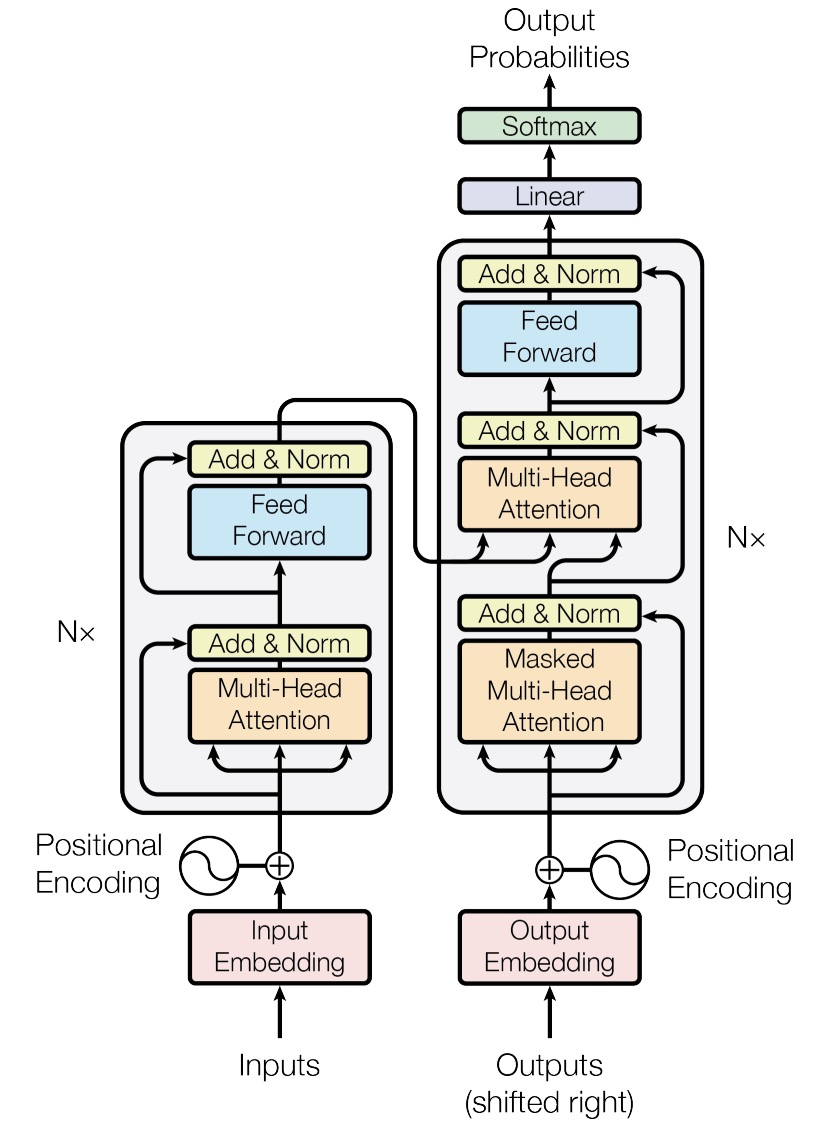
\includegraphics[width=4in]{figures/xulun/transformer.jpg}
  \caption{Transformer 结构框架\cite{vaswani2017attention}。}
  \label{fig1:transformer}
  \end{figure}
  Transformer 是一个基于注意力机制,特别是自注意力机制的模型,
  从根本上摒弃了传统的循环神经网络(RNN)和卷积神经网络(CNN)。
  如\figref{fig1:transformer}, 
  Transformer 模型包含两个
  主要部分:编码器(图左侧)和解码器(图右侧)。这两部分均由数个结构一致的层组成,其
  中每一层都融合了自注意力机制和前馈神经网络。

  \textbf{编码器的介绍}

  Transformer的编码器部分由六个相似的层构成,每层包括两个主要子结构:
  \begin{itemize}
    \item 多头自注意力机制:作为编码器的核心,这一机制使得模型在处理序列中的每个元素时能同时关注其他元素,从而深刻理解整个序列的上下文关系。
    \item 逐位置的前馈网络:这个全连接网络层对序列中每个位置的数据进行独立的线性变换,进一步加强了模型对位置信息的处理能力。
  \end{itemize}
  此外,编码器的每个子层均采用残差连接和层归一化策略,有效防止了深层网络中梯度消失问题的发生,保障了信息的流畅传递。
  
  \textbf{解码器的介绍}

  解码器部分的结构与编码器相似,也是由六个层组成,但在子结构上有所不同,主要包括:
  \begin{itemize}
    \item 掩码多头自注意力机制:与编码器类似,但增加了掩码功能,防止解码器在生成序列时提前获取未来的信息,从而确保了信息生成的时序性。
    \item 编码器-解码器注意力:这一机制使解码器能够关注编码器的所有输出,为序列的生成提供了完整的输入序列上下文。
    \item 逐位置的前馈网络:与编码器的前馈网络相同,它独立处理序列中每个位置的信息。
  \end{itemize}
  解码器的每个子层同样使用残差连接和层归一化,增强了模型的稳定性和训练效率。

  \textbf{缩放点积注意力(Scaled Dot-Product Attention)}

  在Transformer模型中,\textit{缩放点积注意力}(Scaled Dot-Product Attention)起
  着核心作用。它通过计算\textit{查询}($Q$)和\textit{键}($K$)之间的点积,
  来量化序列元素间的关联程度。为了在高维空间中保持梯度的稳定,缩放点积注意力机制将
  点积结果除以\textit{键}的维度$d_k$的平方根进行缩放。其数学表达式为:
  \begin{equation}
      \text{Attention}(Q, K, V) = \text{softmax}\left(\frac{QK^\top}{\sqrt{d_k}}\right)V
  \end{equation}
  其中$V$代表\textit{值}(Value),而softmax函数确保输出的归一化。这种设计使
  得每个元素的输出成为输入值的加权和,其中权重反映了元素间的相关性。
  
  这个机制不仅提升了Transformer在处理长距离依赖问题上的能力,其并行计算特性
  也大大提高了模型的效率。

%\textbf{自注意力机制(Self-Attention)}
%是Transformer结构的基石,它允许模型在处理序列的每个元素时,考虑到序列中的所有其他元素。自注意力的计算公式如下:
%\[ \text{Attention}(Q, K, V) = \text{softmax}\left(\frac{QK^T}{\sqrt{d_k}}\right)V \]
%其中,\(Q\)、\(K\)、\(V\) 分别表示查询(Query)、键(Key)和值(Value),\(d_k\) 为键的维度。

%\textbf{缩放点积注意力(Scaled Dot-Product Attention)}是自注意力机制的一种具体实现,通过缩放因子调整查询和键的点积计算。它提供了一种有效的方法来评估输入元素间的相似度。缩放点积注意力的公式为:
%\[ \text{Scaled Dot-Product Attention}(Q, K, V) = \text{softmax}\left(\frac{QK^T}{\sqrt{d_k}}\right)V \]

\textbf{多头注意力(Multi-Head Attention)}

多头注意力机制是Transformer架构中的一个关键创新,它的设计旨在使模型能够同时从
不同的表示子空间捕获信息。这一机制的核心在于,它不是单一地应用注意力机制,而是将其
分解为多个并行的``头'',每个头独立地关注输入数据的不同方面,从而提高了模型整体的处理能
力和灵活性。

在多头注意力机制中,每个头都独立地执行缩放点积注意力的操作。这一过程可以分为以下几个步骤:

\textbf{头的分割与独立运算}:输入的查询($Q$)、键($K$)和值($V$)首先被分割成多个头,每个头对应一组不同的权重矩
阵 $W_i^Q$、$W_i^K$ 和 $W_i^V$。这些权重矩阵是模型中的可学习参数,用于将输
入映射到相应的子空间中。其中每个头的计算公式为:
\begin{equation}
\text{head}_i = \text{Attention}(QW_i^Q, KW_i^K, VW_i^V)
\end{equation}

\textbf{缩放点积注意力}:已经介绍过。在每个头中,我们对映射后的查询、键和值执行缩放点积注意力计算。
这包括计算查询和键的点积,根据键的维度进行缩放,应用softmax函数获取注意力权重,最后用
这些权重加权求和值。

\textbf{拼接与输出映射}:计算完所有头的缩放点积注意力后,将它们的输出拼接起来,
再通过一个额外的权重矩阵 $W^O$ 进行映射,得到最终的输出:
\begin{equation}
\text{MultiHead}(Q, K, V) = \text{Concat}(\text{head}_1, \text{head}_2, \dots, \text{head}_h)W^O
\end{equation}

多头注意力机制的引入,使Transformer模型能够同时捕获序列的不同特征(如语法、语义等),
并处理各种复杂的依赖关系。这种机制的优势在于其并行性和灵活性,使得模型在处理复杂的序列任
务时更加高效和准确。

通过这种细致的解释,我们可以更深刻地理解多头注意力机制的工作原
理及其在Transformer模型中的重要作用。这种机制不仅是Transformer的核心创新之一,
也是推动当前自然语言处理领域发展的关键技术。

%多头注意力机制通过将自注意力分解为多个``头'',在不同的表示子空间中并行执行,从而捕捉输入数据的多样化特征。多头注意力的计算公式为:
%\[ \text{MultiHead}(Q, K, V) = \text{Concat}(\text{head}_1, \text{head}_2, \dots, \text{head}_h)W^O \]
%其中,每个头 \(\text{head}_i\) 的计算为 \(\text{Attention}(QW_i^Q, KW_i^K, VW_i^V)\),\(W_i^Q\)、\(W_i^K\)、\(W_i^V\) 和 \(W^O\) 是模型中的可学习权重矩阵。
%
%Transformer模型通过其创新的自注意力机制和编码器-解码器架构,为处理复杂的自然语言任务提供了强大的工具。

\subsubsection*{2) Transformer的衍生模型}

随着NLP技术的不断进步,Transformer的衍生模型,如BERT、GPT、XLNet和RoBERTa,
将Transformer结构与无监督学习结合,
可以在不同NLP任务上实现前所未有的性能,无需每个任务重新训练。
这些模型可根据使用的Transformer结构分类:

\begin{equation*}
  \text{衍生模型} \left\{
      \begin{array}{l}
        \text{Encoder模型(如BERT、RoBERTa),称为自编码模型。} \\ 
        \text{Decoder模型(如GPT、XLNet),称为自回归模型。}
      \end{array}
  \right.
\end{equation*}




\subsubsection*{Encoder模型}

Encoder 模型只使用 Transformer 模型中的 Encoder 模块,也被称为
自编码(auto-encoding)模型。在每个阶段,注意力层都可以访问到原始输入
句子中的所有词语,即具有``双向''注意力。
Encoder 模型通常通过破坏给定的句子(例如随机遮盖其中的词语),
然后让模型进行重构来进行预训练,最适合处理那些需要理解整个句子语义的任务,
例如句子分类、命名实体识别(词语分类)、抽取式问答。
BERT 是第一个基于 Transformer 结构的纯 Encoder 模型,它在提出
时横扫了整个 NLP 界,在流行的 GLUE 基准上超过了当时所有的最强模型。
随后的一系列工作对 BERT 的预训练目标和架构进行调整以进一步提高性能。
目前,纯 Encoder 模型依然在 NLP 行业中占据主导地位。下面简略介绍一下 
BERT 模型及它的变体RoBERTa。

\subsubsection*{BERT 模型}

BERT是基于 Transformer 架构的自然语言处理模型。它采用 Transformer 的编
码器部分来学习文本中单词或子单词之间的上下文关系。与传统的单向模型不同,
BERT 的编码器一次性读取整个单词序列,因此,虽然通常被描述为``双向''模型,
但更准确地说,它是非定向的。

BERT 的训练涉及两种主要策略:Masked LM (MLM)和Next Sentence Prediction (NSP)。
Masked LM (MLM)是在输入序列中随机选择大约15\%的单词并用特殊的[MASK]标记替换,然
后模型尝试预测这些被遮盖的单词。这需要在编码器的输出顶部添加一个分类层,并且通过词嵌入矩
阵将输出向量转换为词汇量,最后使用 softmax 函数计算每个单词的概率。BERT 的损失函数
仅考虑遮盖值的预测。

Next Sentence Prediction (NSP)策略是BERT 接受成对的句子作为输入,并学习预
测第二个句子是否逻辑上紧跟在第一个句子之后。在输入中,50\%是连续的句子对,另一
半则是随机的句子对。在输入模型之前,每个输入序列的开始位置会添加一个特殊的[CLS]标记,
每个句子的末尾添加[SEP]标记,同时引入句子嵌入和位置嵌入。为了预测第二个句子是否跟随
第一个句子,模型将[CLS]标记的输出转换为一个二维向量,并使用 softmax 计算其为连续句子的概率。

BERT 在多个基准测试上取得了显著的成绩,包括 
GLUE、SQuAD、SWAG\cite{zellers2018swag}、CLOTH\cite{xie2018large}、
DREAM\cite{sun2019dream}和 SQuAD 2.0。
BERT 通过这种方式,在理解语言的多个方面,尤其是上下文理解方面,取得了新的突破。然而,由
于其复杂的结构和依赖于大量数据的特点,BERT 在一些情况下难以解释,并且在处理特定类型的
语言数据时可能存在泛化问题。尽管如此,BERT 仍然是自然语言处理领域的一个重要里程碑,并
为后续的模型如 XLNet、RoBERTa 等奠定了基础。

\subsubsection*{RoBERTa 模型}
RoBERTa 模型代表了在深度学习和自然语言处理领域中对
BERT模型的一个重要的进化步骤。这种进化不仅基于对BERT潜力的深入挖掘,而且体
现了对预训练语言模型的深刻理解。在这一过程中,RoBERTa的开发者们采用了四个创
新和优化措施,旨在全面提升模型的性能和适应性。

首先,关于数据集的扩展和训练时长的增加,这些改变源于一个核心理念:更多的数据和
更长的训练周期能够使模型捕捉到更为复杂和微妙的语言模式。通过将数据量从BERT的16GB增
加到160GB,并将训练迭代次数从100K提升至500K,RoBERTa能够在更广泛和多样化的文本上学
习,从而提升其对于复杂语言结构的理解能力。

动态掩码的引入是RoBERTa另一个创新之处。与BERT的静态掩码不同,RoBERTa在每个epoch
中对文本采用不同的掩码模式。这种方法有效防止了模型对固定掩码模式的过度适应,从而推动模型
学习更加泛化的语言表示。具体而言,这种动态掩码策略是在训练过程中实时应用的,确保即使同一
文本在不同的训练阶段也会呈现出不同的掩码模式,增加了训练的多样性和复杂性。

此外,去除BERT中的下一个句子预测(NSP)任务也是一个关键决策。尽管NSP被设计来提高模型
对句子间关系的理解,但研究发现,在去除这一任务后,RoBERTa在多项下游任务中的表现有了显
著提升。这表明对于模型的优化,有时候减法也是一种有效的策略。

再者,RoBERTa在训练中对样本长度的处理也展示了其对复杂语言模式理解的重视。通过在训
练中始终使用全长(512个令牌)的序列,RoBERTa强化了对长距离依赖关系的学习,这对于
处理更为复杂的语言结构至关重要。

这些改进使得 RoBERTa 在多个基准测试(如 GLUE、RACE\cite{lai2017race}、SQuAD 等)
中取得了领先性能,甚
至超过了人类的表现。
综合来看,RoBERTa的这些创新和优化措施共同构成了其卓越性能的基础。通过在大规模数据
集上进行深入训练,实施动态掩码机制,精简训练任务,以及优化样本长度处理,RoBERTa不仅
巩固了BERT作为一种强大的语言模型的地位,也为后续的NLP研究提供了宝贵的参考和启示。


\subsubsection*{Decoder模型}
Decoder 模型只使用 Transformer 模型中的 Decoder 模块。在每个阶段,对
于给定的词语,注意力层只能访问句子中位于它之前的词语,即只能迭代地基于已经生
成的词语来逐个预测后面的词语,因此也被称为自回归(auto-regressive)模型。
下面就简要介绍一些常见的Decoder 模型。

\subsubsection*{GPT 模型}
GPT 模型是第一个使用了Transformer架构进行预训练的大型语言生成模型。这个模型标志着自然语言处
理中一个重要的转变点。
GPT 结合了 Transformer Decoder 架构和迁移学习方法,
在大量开放在线数据上进行无监督预训练,特别是在 BookCorpus 数据集上。
其预训练任务是根据上文预测下一个单词,从而使模型能够在没有限制的情况下学习语言特征。
此外,GPT 还通过微调适应各种下游任务,如文本蕴含、语义相似性、情感分析等,在包括
SNLI、MNLI、ROC、COPA 和 GLUE 等多个 NLP 基准
测试中取得了显著效果。

然而,GPT 也存在一些局限性,比如它主要使用单向(向前)自注意力机制,这意味
着在处理文本时,每个词只能看到它前面的词,这限制它对上下文的理解。

\subsubsection*{XLNet 模型}
XLNet 模型也基于Transformer Decoder架构,但采用了双向
(或更准确地说是排列敏感的)上下文处理。XLNet通过排列语言
建模(Permutation LM)来同时学习文本的前向和后向依赖。
XLNet的出现在自然语言处理领域引发了显著关注,特别是它在
特定任务中相较于BERT的显著性能提升,标志着NLP模型发展的一个新阶段。这种
模型不仅继承了自回归语言模型的强大特性,同时也融合了自编码语言模型(如BERT)的优
势,创造了一种新的、更为复杂和有效的预训练机制。

XLNet的核心在于它的创新性预训练目标——排列语言模型。在
BERT中,模型预训练是通过随机选择一些单词并将其替换为[MASK]标记来进行的,
然后模型被训练来预测这些被掩盖的单词。然而,这种方法导致了一个问题:在实
际应用中,即微调(fine-tuning)阶段,输入数据中并不存在[MASK]标记,这可
能导致预训练和微调之间的不一致性。
为了解决这个问题,XLNet引入了排列语言模型。在这种模型中,对于一个给定长度
的句子,模型会考虑所有可能的单词排列组合。在每次训练迭代中,
模型会随机选择一种排列,并基于这种排列来预测单词。具体来说,对于一个句子中
的每个位置,
模型尝试预测这个位置的单词,给定在这个特定排列中它之前的所有单词。
这种方法有效地模拟了自回归(autoregressive)语言模型的特性,
同时也使模型能够在预训练中学习到上下文的全面信息。

在与BERT的比较中,XLNet的预训练机制展现出三个独特的优势:
首先,BERT通过在输入中随机遮盖某些词并预测这些词来进行训练,而
XLNet则采用了无需明显[MASK]标记的内部随机``遮盖''单词方法。这种差异使得
XLNet在预训练和微调阶段保持了更高的一致性,解决了BERT预训练与微调不一致的问题。

此外,XLNet在处理生成型任务上也表现出明显的优势。得益于其自回归特
性,XLNet能够在维持自然的从左到右的生成过程的同时,内部隐含上下文信
息,这对于生成连贯、流畅的文本尤为重要。

针对长文本的处理能力也是XLNet的一个亮点。它整合了
 Transformer XL\cite{dai2019transformer} 的技术,使
得在处理长文档类型的NLP任务时,相比BERT有着更为显著的优势。

总的来说,XLNet通过结合自回归和自编码语言模型的优势,通过其排列语言模型和注
意力掩码机制,有效地利用上下文信息。这些特性使得XLNet在多项NLP任务中,尤其是在
生成型任务和长文档处理方面,相较于BERT展现出更加卓越的性能。这种创新的预训练方法
不仅解决了先前模型的某些局限性,也为未来NLP模型的发展提供了新的方向。


\subsection{推理模型鲁棒性研究}
\label{sec1:robustness}
上一小节是我对我所研究的相关的推理方法的介绍,尽管大型预训练语言模型在NLP
领域取得了显著进展并
在现实世界中得到了广泛应用,
但它们在处理领域外数据、抵御对抗性攻击\cite{mccoy2019right,jin2020bert}以及应对输入的微
小扰动\cite{ebrahimi2018hotflip,belinkov2018synthetic}方面仍显脆弱。这些局限性
可能会阻碍这些模型在实际环境中的安全部署,并影响用户对NLP模型的信任度。为了应对这些
挑战,语言技术领域的研究者们正加大力度,旨在深入理解并解决这些鲁棒性问题。
在这一节中,我们将进一步讨论自然语言推理任务中模型鲁棒性的相关研究。
%接下来是对这些模型在具体任务上的鲁棒性的探究的相关工作,
包括模型的鲁棒性的测试和提高模型鲁棒性的相关方法。

\subsubsection{鲁棒性的定义和评估方法}

Wang等人(2022)\cite{wang2022measure}对模型的鲁棒性进行了定义:

\begin{definition}[鲁棒性]
在自然语言处理模型中,\textbf{鲁棒性}指的是模型在面对不同分布的测试数据时保持性能的能力。
具体来说,对于一个输入 $x$ 和它的正确标签 $y$,对于一个在 $(x, y) \sim D$ 上训练的模型 
$f$ 及其对 $x$ 的预测 $f(x)$,鲁棒性是通过模型在测试数据 
$(x', y') \sim D'$(可能与 $D$ 分布不同)上的表现来衡量的。
通常使用诸如鲁棒准确率这样的指标来量化鲁棒性,
定义为 $E_{(x', y') \sim D'}[f(x') = y']$。
\end{definition}

在探讨模型鲁棒性的文献中,可以粗略地将他们分为两类:对抗性攻击下的鲁棒性和分布偏移下的鲁棒性。
对抗性鲁棒性关注在输入 $x$ 周围创建微小扰动 $\delta$ 形成 $x'$ 时模型的表现,
而分布偏移鲁棒性关注在自然发生的不同分布上的模型表现。
这些分类共同探讨 $D'$ 是合成分布偏移(如对抗性攻击)还是自然分布偏移。

\textbf{对抗性攻击下的鲁棒性}:
对抗性鲁棒性的研究主要集中在模型对输入的微小扰动($\delta$)的反应上,
即在原始输入 $x$ 周围引入扰动,形成 $x'$,并观察模型的响应。这类攻击通常通过添加
对人类几乎不可察觉的噪声,以欺骗模型做出错误判断。这种策略最初在计算
机视觉领域被广泛研究\cite{szegedy2014intriguing,goodfellow2014explaining},
随后扩展到自然语言处理领域\cite{Marco2020acl,tan2020s,schwinn2023exploring,boucher2022bad},
凸显了对NLP模型进行全面鲁棒性评估的重要性。

\textbf{分布偏移下的鲁棒性}:
与之相对,分布偏移下的鲁棒性关注模型在不同自然分布的数据上的表现。
这类研究反映了现实世界数据多样性和复杂性的影响,如语法错误、方言、
语言差异等因素\cite{blodgett2016demographic, demszky2021learning},以及
同一任务在不同领域的新数据集上的表现。


CheckList\cite{Marco2020acl}是一个结合了对抗性攻击和分布偏移下鲁棒性测试的方法论。
它借鉴软件工程中的``黑盒测试''方法,重点评估NLP模型在不同输入变化下的表现。这一方法论包括三
个核心部分:功能评估、测试方法和测试用例生成。

1)功能评估:此部分更多关注模型在处理各种NLP任务(如语义角色标注、命名实体识别等)时的能力,
为后续的鲁棒性测试奠定基础。

2)测试方法和测试用例:这里包括对抗性攻击下的鲁棒性和分布偏移下的鲁棒性两个方面。
对于前者,CheckList通过模拟对抗攻击中的微小变化或扰动(如情感分析中的句子轻微修改),
评估模型的反应\cite{goodfellow2014explaining}。它通过不变性测试(INT)和定向期望测试(DIR)等方法,
检验模型在处理对抗性攻击下的鲁棒性(如语法结构变化、情感强度变化)时的稳定性。同时在分布偏移的鲁棒性的测试中,
CheckList通过模板方法简化了大量有效测试用例的创建。
例如,可以创建一个模板``我\{NEGATION\}\{POS\_VERB\}这个\{OBJECT\}'',
并通过不同的词语组合生成多个测试句子,如``我不喜欢这个电影'',来评估模型对否定构造的处理能力。这些例子的主题和分布与原来的测试集已经完全不同。

总结来说,CheckList为NLP领域提供了一个全面的框架,
用于评估和提升模型在面对对抗性攻击和分布偏移时的鲁棒性。
这不仅有助于揭示模型的潜在薄弱环节,也为提高模型的整体鲁棒性提供了实践指导。

\subsubsection{提升推理模型鲁棒性的方法}
在自然语言推理的领域中,关键的目标之一是增强模型的鲁棒性。为此,我们通常采
用两种主要策略:一是数据增强技术,用于丰富训练材料;二是优化模型架构和训
练流程,以提升模型的内在强度和适应能力。

1) 数据增强,作为优化大规模神经网络模型性能的核心策略,
在自然语言处理领域的应用尤为关键。我们概述了几种主要的文本数据增强技术及其在学术研究中的应用,
展示了它们如何为自然语言推理任务带来显著的性能提升。

\textbf{回译(Back-translation)}\cite{sennrich2016improving,edunov2018understanding,xie2020unsupervised}:
通过将文本从一种语言翻译到另一种语言,再翻译回原语言,创造出文本的新变体,从而增加数据的多样性。

\textbf{c-BERT词替换}\cite{wu2019conditional}:
运用BERT模型来识别并替换文本中的关键词汇,生成文本的新版本,以此来丰富语料库。

\textbf{混合(Mixup)}\cite{guo2019augmenting,chen2020mixtext}:
通过在不同文本样本之间进行线性组合,创造全新的文本实例。

\textbf{截断(Cutoff)}\cite{shen2020simple}:
分为两类,第一类叫做Token截断,即随机选取Token,将对应Token的嵌入整行置零;第二类是特征截断,
即随机选取嵌入的特征,将所选特征维度整列置零。

2) 优化模型架构和训练流程的方法,一般指的是调整模型结构来增强模型在自然语言推理任务当中的鲁棒性。
最常用的方法是\textbf{对抗性训练}\cite{zhu2019freelb,jiang2020smart},
这种方法通过在词嵌入层引入微小的扰动,合成附加样本,提高模型对异常输入的鲁棒性。
该方法通过梯度反传生成对抗性扰动,并加到原始嵌入矩阵上,产生增强样本,
通常应用于有监督训练场景。

在Qu(2020年)\cite{qu2020coda}的研究中,通过比较这些模型增强技术
在RoBERTa模型上处理自然语言推理任务(MNLI)的效果,发现回译和对抗性训练在提升模型
性能方面效果显著,明显优于c-BERT、混合和截断技术。因此,将回译作为自然语言推理任务中的一
种强有力的基准进行数据增强方法比较,是一种合理的策略。这些研究成果不仅强调了数据增强在提
升模型性能方面的重要性,还为选择适当的数据增强策略提供了宝贵的指导。

\subsection{推理模型可解释性研究}
\label{sec1:interpretability}

\subsubsection{推理模型鲁棒性不足的现象}

在本节中,我们聚焦于推理模型在处理常识性推理任务时所表现出的鲁棒性不足问题。虽
然这些模型在标准测试环境中取得了显著成就,但它们在遭遇对抗性数据或与训练环境
显著不同的场景时,却显露出不足\cite{naik2018stress,mccoy2019right,schuster2019towards,nie2020adversarial,Marco2020acl}。

以CheckList\cite{Marco2020acl}为例,该研究通过对模型进行重新测试,涵盖
了多种不同能力,结果显示模型性能与原始测试结果相比有显著
差异。这一发现揭示了模型在鲁棒性方面的严重不足。然而,尽管CheckList在揭露
模型学习过程中的一些缺陷上取得了进展,比如在``语义角色标注''等任务下的表现,
它却未能深入分析导致模型鲁棒性不足的根本原因。

\subsubsection{推理模型鲁棒性不足的原因的探究}

在深入探究推理模型鲁棒性不足的问题时,关键在于分析模型处理信息的方式和焦点。
一种常见的假设是,这些模型可能过于专注于数据的特定结构元素,例如,它们可能
只关注\textit{前提}-\textit{假设}关系对中的\textit{假设},而忽视了前提与假设之间的逻辑联系。这种假设揭示了一个更深层
次的问题:模型可能主要学习了数据中的
统计偏差\cite{naik2018stress,mccoy2019right,schuster2019towards,nie2020adversarial},
也就是所谓的偏见线索(bias cues)或虚假线索(spurious cues)。

这种现象的根源在于数据集的构建方式。由于数据集的特定特征或模式,模型往往不是
学习解决问题的通用策略,而是学习特定于该数据集的简化规则。举个例子,在自然
语言处理任务中,如果某个数据集中绝大多数标记为``正确''的样本都包含某个特定的词汇,模型
可能就会简单地依赖这个词汇来做出判断,而没有真正理解句子之间的逻辑关系。这种简化的
学习方式使模型在面对结构或上下文有所不同的新数据时显得脆弱,无法有效适应或正确解释。
如果这种线索刚好在\textit{假设}部分,
那可能就会造成模型只关注\textit{假设}部分。

因此,探究推理模型的鲁棒性不足,我们不仅要关注模型本身的处理机制,也需要深入理解数据
集构建的影响。


\subsubsection{推理模型鲁棒性不足的原因的验证}

在前面探讨推理模型鲁棒性不足的原因时,研究人员提出了一个关键假设:
模型可能过分专注于数据的特定结构元素,如仅关注推理任务中\textit{假设}部分而忽略了\textit{前提}。
为了验证这个假设,研究者们开发了``仅假设''测试\cite{gururangan2018annotation}和注意力图\cite{vig2019multiscale}这两种方法,
旨在深入分析验证和量化此现象。

\subsubsection*{仅假设测试}

``仅假设''测试的核心思想是检验模型在仅凭假设(即问题或选项本身)的情况下的表现。
这种测试通常用于评估自然语言理解模型。在这种测试中,模型只被提供假设部分,而没
有相应的前提或上下文信息,比如在 \secref{sec1:challenge} 中提到的SNLI的例子,只提供假设
``A man is pushing a baby carriage'' 而不提供前提,让模型猜测前提跟假设之间的关系。
从人的角度来看,
解决这个问题是不可能的,因为问题本身有缺陷,很难做出选择,但是如果模型依然做出跟有前提时一致的结果,
研究者就可以判断模型可能过度依赖于假设中的某些关键词或短语,而忽
略了理解整体意义所必需的上下文。

这种方法的主要优势在于能够揭示模型潜在的缺陷:模型可能
仅依赖假设中的关键信息来作出判断,而不是实现全面的理解。然而,其局限性
在于它不能完全展现模型在处理真实场景时的推理模式。这是因为模型在训练阶段所
依赖的数据包含了前提,而在测试时使用的数据结构却与之不同,仅包含假设而无前提。这
种结构变化导致的差异和信息损失是该方法无法克服的。

\subsubsection*{注意力图}

注意力机制是深度学习中的一种重要技术,它帮助模
型聚焦于输入数据的关键部分。注意力图是一种可视化工具,它展示
了模型在做出决策时对不同输入部分的关注程度。通过观察这些图,研究者
和开发者可以更直观地理解模型的决策过程,识别模型关注的是哪些信息。

然而,注意力图的直观性并不总是代表其可靠性或准确性。
研究\cite{jain2019attention}指出,即使模型通过注意力机制
突出显示的部分,也可能并不准确地代表模型决策的真实依据。这表明,
尽管注意力图提供了一个理解模型决策过程的窗口,但它不应被视为模
型内部工作机制的完整映射。

虽然``仅假设''测试和注意力图作为工具在解析和评估模型行为方面扮演着关键角色,
但它们的分析深度有限。这些方法虽然能在一定程度上揭示模型中的偏见,但在深入探讨数
据中的偏见如何影响模型的核心机制方面,仍显不足。因此,对数据偏见如何具体作用于模型
的机制进行深入研究,已成为当前一个亟待解决的重要课题。



\subsection{本章小结}

在本章中,我们全面而深入地探讨了常识性推理领域的核心要素。章节始
于对该领域的基本任务和评估标准的深度分析,揭示了其核心内容、目标和所面
临的挑战。随后,我们对推理模型的发展历程进行了细致的梳理,从符号方法、早
期统计方法,一直到神经网络方法,并对这些方法的优势和局限性进行了详尽的讨论。特
别地,对于常识性推理中的神经网络方法,我们进行了深入的阐述,这些方法和模型将在后
续章节中反复出现和引用。

章节接下来转向推理模型鲁棒性的研究,详细探讨了鲁棒性的定义、测试
方法,以及提升模型鲁棒性的多种策略。我们对模型在处理多样化和对抗性
数据时的挑战进行了深入的剖析,并探索了增强模型适应性和鲁棒性的有效方法。
最终,本章还深入讨论了推理模型的可解释性研究,特别是模型鲁棒性不足的表现、原
因的假设以及这些假设的验证方法。

综合来看,本章旨在为读者提供一个全景式的视角,深刻理解常识性推理领域的最
新研究趋势和发展,包括其核心任务、评估基准、方法论以及鲁棒性和可解释性研究的最新进展。

\newpage
\null
\newpage